\section{Methodology}

\subsection{Overview}

In this project, we undertook the integration of various sensors to enhance predictive maintenance capabilities. The key components and methodologies involved in each sensor type are summarized below:

\begin{itemize}
  \item \textbf{Temperature Sensors:}
    \begin{enumerate}
      \item Identification of specific data requirements for bearing temperature.
      \item Selection of contact-type temperature sensor.
      \item Integration into the data acquisition system.
      \item Calibration and rigorous testing to ensure accuracy.
    \end{enumerate}

  \item \textbf{Current Sensors:}
    \begin{enumerate}
      \item Comprehensive understanding of current sensing principles.
      \item Selection of appropriate current sensor type.
      \item Incorporation into the system architecture.
      \item Validation and testing under various conditions.
    \end{enumerate}

  \item \textbf{Vibration Accelerometers:}
    \begin{enumerate}
      \item Deep understanding of vibration accelerometer operation.
      \item Selection of suitable accelerometer type utilizing the piezoelectric effect.
      \item Integration into the system and implementation of signal processing techniques.
      \item Exploration and implementation of machine learning algorithms.
      \item Establishment of continuous monitoring for proactive maintenance.
    \end{enumerate}
\end{itemize}

The successful execution of these methodologies has significantly enhanced our system's capabilities for efficient data acquisition, analysis, and proactive maintenance in industrial applications.


\subsection{Data Collection}

The systematic collection of temperature and current data from a motor involved creating a time-ordered series of data points. Measurements of temperature and current were meticulously taken at regular intervals to establish a comprehensive dataset for analysis and monitoring.

\subsubsection{Temperature Sensor}

\begin{figure}[!h]
	\centering
	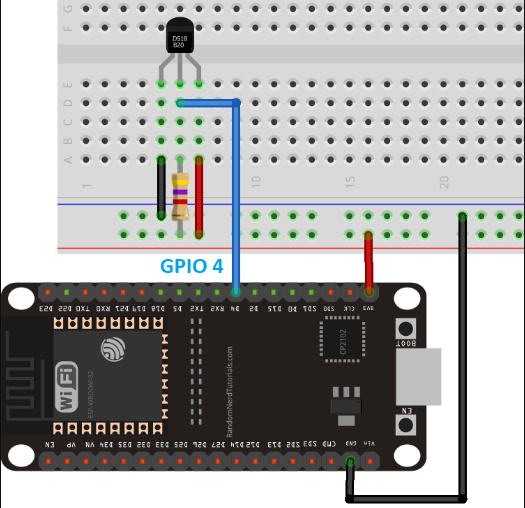
\includegraphics[width=0.7\linewidth, height=8cm]{Figures/ds18b20}
	\caption{ds18b20 Pin Out}
\end{figure}

To initiate a temperature measurement and conversion, a command for reading and conversion is issued to the ds18b20 sensor. Following the conversion process, the resulting thermal data is stored in the 2-byte temperature register in the scratchpad memory. It is crucial to note that for the execution of this command, an external power supply is utilized to specify read time slots, ensuring the reliability and accuracy of the temperature readings.

\subsubsection{Current Measurement}

In parallel with temperature data collection, current measurements were acquired using appropriate sensors designed for the motor's electrical system. These sensors provided real-time information on the electrical load and power consumption, contributing essential data for comprehensive motor health analysis.

The combination of temperature and current data forms the foundation for subsequent analysis, enabling proactive maintenance and effective decision-making regarding the motor's operational status.


\pagebreak 

\begin{lstlisting}
	void loop() {
		sensors.requestTemperatures(); 
		float temperatureC = sensors.getTempCByIndex(0);
		float temperatureF = sensors.getTempFByIndex(0);
		Serial.print(temperatureC);
		Serial.print(temperatureF);
		Serial.println("F");
		delay(5000);
	}
\end{lstlisting}



\begin{figure}[!h]
	\centering
	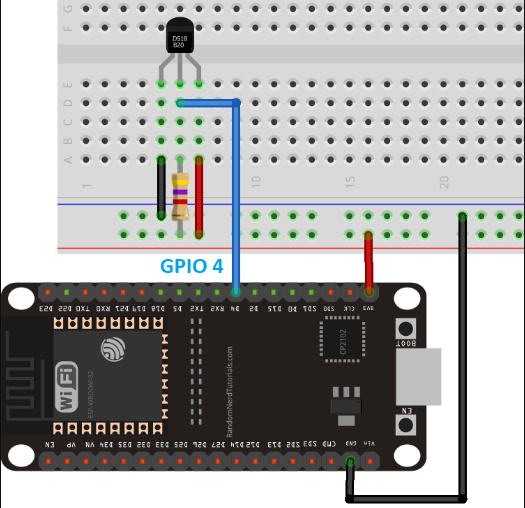
\includegraphics[width=0.7\linewidth, height = 8cm]{Figures/ds18b20}
	\caption{current sensor pin out}
	
\end{figure}
Current flows through the onboard hall sensor circuit in its IC
The hall effect sensor detects the incoming current through its magnetic field generation
Once detected, the hall effect sensor generates a voltage proportional to its magnetic field that’s then used to measure the amount of current 

\subsection{Vibration Analysis}

In order to ascertain the natural frequency of a system and predict potential resonance occurrences, a comprehensive understanding of the system's mass, stiffness, and damping characteristics is essential. Resonance manifests when the excitation frequency aligns with the natural frequency of the system, resulting in a significant amplification of vibration amplitudes. The following outlines the methodology for determining natural frequency and identifying resonance conditions:

\begin{figure}[!h]
	\centering
	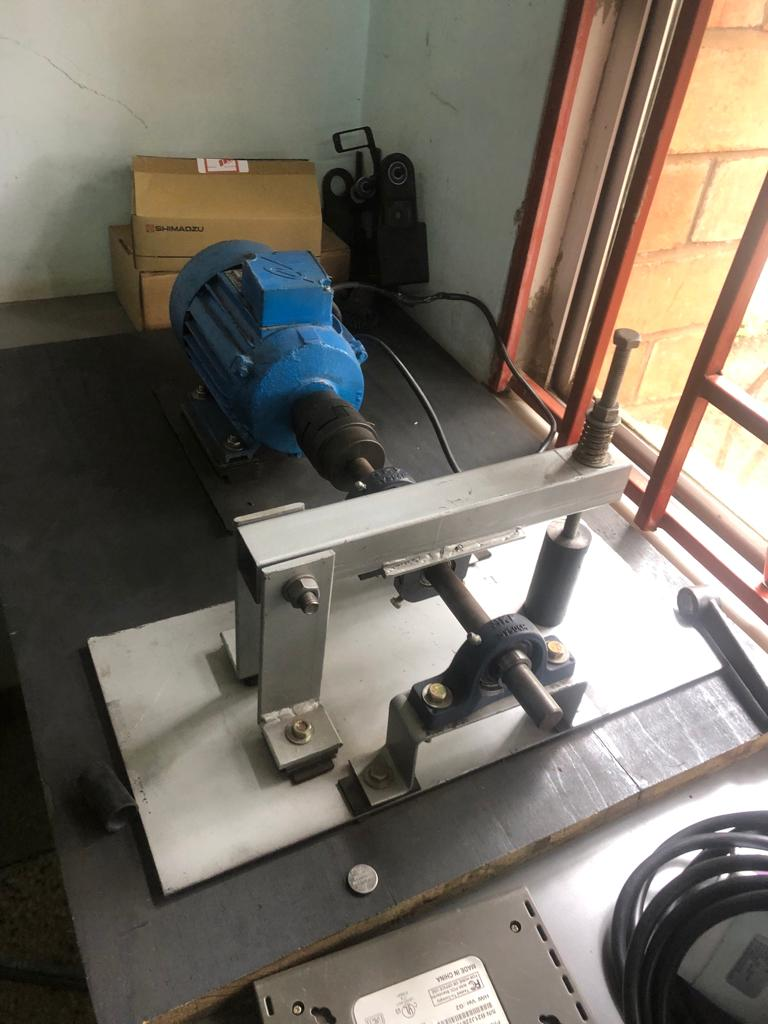
\includegraphics[width=0.7\linewidth, height=8cm]{Figures/motor_mount}
	\caption{Vibration Sensor Setup}
\end{figure}

Firstly, the mechanical system under consideration is meticulously modeled, with a precise definition of the mass, stiffness, and damping properties of its components. This representation can be achieved through mathematical equations or software tools such as finite element analysis (FEA), ensuring a comprehensive understanding of the system's dynamic behavior.

Subsequently, an eigenvalue analysis or modal analysis is conducted on the system model. This analytical process calculates the natural frequencies and mode shapes of the system, elucidating the vibration patterns associated with each natural frequency. The identification of the natural frequency linked to the mode of interest is pivotal, as it determines the specific vibration behavior under examination.

Furthermore, recent advancements in vibration analysis techniques involve the utilization of machine learning algorithms to enhance the accuracy of resonance prediction and provide insights into complex vibration patterns. This integration of data-driven approaches contributes to a more nuanced understanding of system dynamics and aids in the proactive identification of potential resonance challenges in real-world applications.


\begin{lstlisting}
	// The on-board ADC is 10-bits 
	// Different power supply will lead to different reference sources
	// example: 2\^{}10 = 1024 -> 5V / 1024 \~{}= 4.88mV
	//          unitValue= 5.0 / 1024.0*1000 ;
	float unitValue= RefVal / 1024.0*1000 ;
	float voltage = unitValue * sensorValue; 
	
	//When no load,Vref=initialValue
	SERIAL.print(``initialValue: '');
	SERIAL.print(voltage);
	SERIAL.println(``mV''); 
	
	// Calculate the corresponding current
	float current = (voltage - Vref) * sensitivity;
	
	// Print display voltage (mV)
	// This voltage is the pin voltage corresponding to the current
	/*
	voltage = unitValue * sensorValue-Vref;
	SERIAL.print(voltage);
\end{lstlisting}
 

\subsubsection{Omnimonitor}

The device is responsible for keeping track of and managing data from different sources as well as managing read and write signals from the sensor to the remotely accessible server  
\begin{figure}[!h]
	\centering
	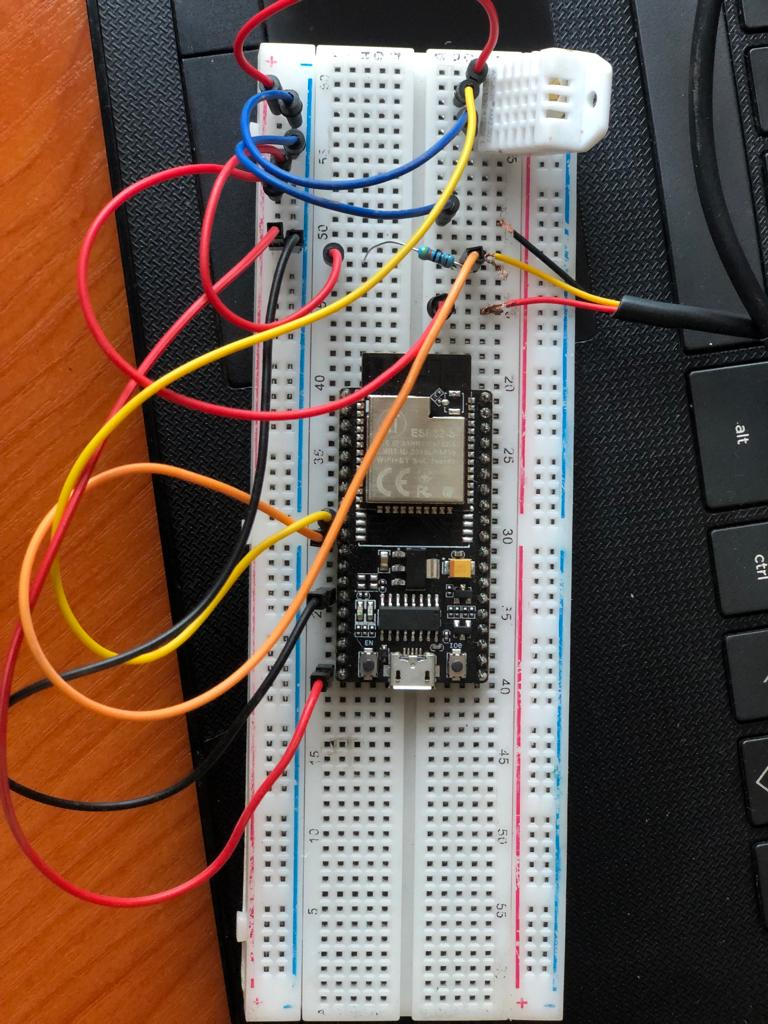
\includegraphics[width=0.7\linewidth, height = 8cm]{Figures/setup}
	\caption{combined sensor setup}
	
\end{figure}
Both ds18b20 and DHT22 provide the output of temperature and humidity in the complex digital output format which can not be directly read with GPIO pins without writing any technique which can read these output signals. These sensors provide data through a single wire two-way communication protocol. A single process communication consists of 40 bits.To get values of temperature and humidity we call a number of created  functions.

\begin{figure}[!h]
	\centering
	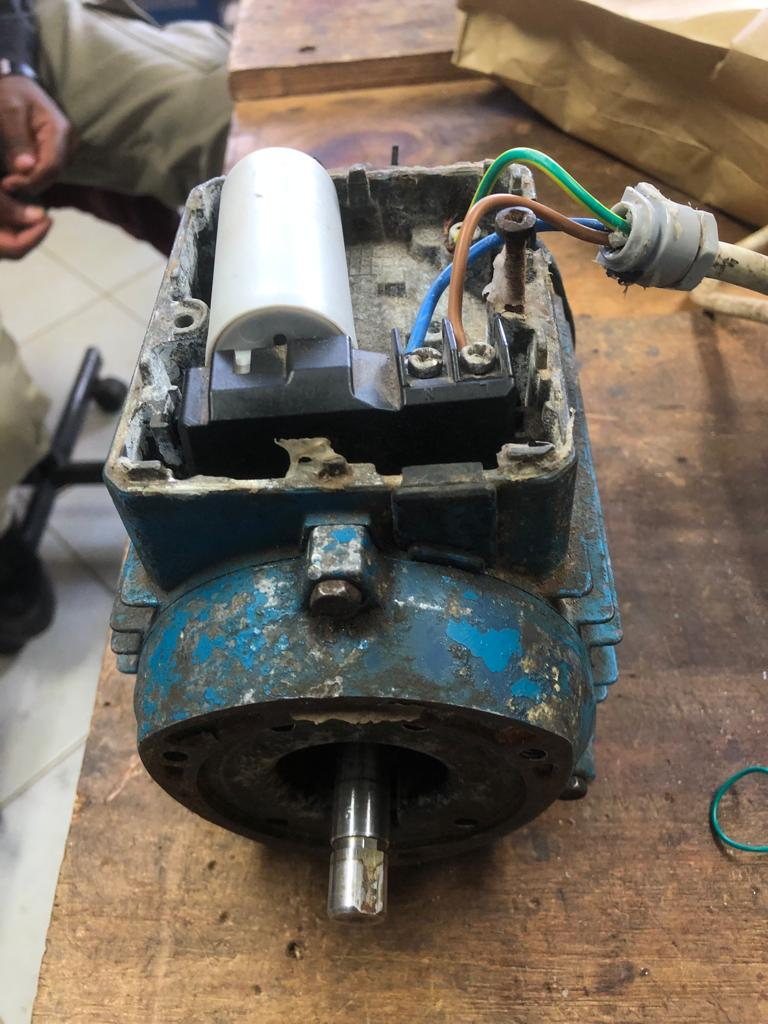
\includegraphics[width=0.7\linewidth, height = 8cm]{Figures/motor.jpeg}
	\caption{sensor setup}
	
\end{figure}

\begin{lstlisting}
	\#if defined(ESP32)
	\#include <WiFiMulti.h>
	WiFiMulti wifiMulti;
	\#define DEVICE ``ESP32''
	\#elif defined(ESP8266)
	\#include <ESP8266WiFiMulti.h>
	ESP8266WiFiMulti wifiMulti;
	\#define DEVICE ``ESP8266''
	\#endif
	

	//\#define DHTTYPE DHT11 // DHT 11
	//\#define DHTTYPE DHT21 // DHT 21 (AM2301)
	\#define DHTTYPE DHT22 // DHT 22 (AM2302), AM2321
	
	// ds18b20 sensor
	\#define ONE\_WIRE\_BUS 26
	OneWire oneWire(ONE\_WIRE\_BUS);
	DallasTemperature sensors(\&oneWire);
	
	uint8\_t DHTPin = 25;
	DHT dht(DHTPin, DHTTYPE);
	
	float temperature\_Celsius; // ambient
	float humidity;
	float temperature\_Celcius2; // contact

	
\end{lstlisting}
	

\subsubsection{MQTT}

Message Queuing Telemetry Transport (MQTT) has proven indispensable in my project focused on predictive maintenance, particularly when dealing with the intricate task of monitoring sensor data from a ship's motor. Operating in maritime environments, where network reliability is often challenged and resources are constrained, MQTT's lightweight messaging protocol serves as a crucial element in establishing efficient machine-to-machine (M2M) communication and seamless integration within the Internet of Things (IoT).

In the implementation phase, We connect my predictive maintenance system to an MQTT broker, which functions as the central hub for communication. This broker efficiently manages the flow of sensor data from the ship's motor, forwarding it to my monitoring and analysis tools. The PUSH/SUBSCRIBE architecture ensures a well-organized and scalable communication framework, a fundamental aspect for real-time monitoring and predictive analysis of the motor's performance.

What sets MQTT apart in this predictive maintenance project is its optimization of data transmission. The protocol's well-defined, compact message structure, featuring a fixed 2-byte header, significantly reduces the communication overhead. In the context of maritime operations, where bandwidth may be limited and latency is a concern, this streamlined approach enhances the speed and responsiveness of data exchanges. The support for Quality of Service (QoS) levels further allows me to fine-tune the balance between message delivery assurance and network performance, a critical consideration for ensuring the timely and reliable transmission of sensor data.

Having successfully implemented MQTT in this predictive maintenance scenario, We've experienced firsthand its effectiveness in navigating through the challenges of low-bandwidth conditions and intermittent connectivity. The protocol plays a pivotal role in facilitating the timely detection of anomalies and potential issues in the ship's motor, enabling proactive maintenance interventions. As the maritime industry increasingly embraces IoT technologies for predictive maintenance, MQTT remains a cornerstone in my toolkit, providing a robust solution for handling sensor data and fostering efficient communication in the dynamic and interconnected environment of predictive maintenance systems for ship systems.


\subsubsection{OTA}

Instead of needing the user to connect the ESP32 to a computer via USB to execute the update, OTA programming allows update of new data to the ESP32 via Wi-Fi.

When there is no physical access to the ESP module, the OTA capability comes in handy. It helps to cut down on the time spent on each ESP module during maintenance.

One of the most useful features of OTA is that it allows a single central location to deliver an update to many equipment on the same network ideally all monitored equipment in a ship engine room.

\subsubsection{Declaration, definition and initialization}

Define, declare variables and initialize classes. 

\begin{lstlisting}
	#define CURRENT_VERSION "1.0.0" // The current version of the firmware running
	#define DOWNLOAD_URL SERVER_URL // The server url where we will get the latest firmware version
	#define DHTPIN 2 // Digital pin connected to the DHT sensor
	#define DHTTYPE DHT11 // DHT 11
	#define LED 4 // Digital pin connected to the inbuilt LED
	WiFiClient espClient; //Initializing the WiFiClient
	void setup_wifi();
	void reconnect();
	PubSubClient client(espClient); // Initializing the PubSubClient
	WebServer server(80); // Initializing the WebServer
	// functions to take care of OTA firmware update
	void handleRoot();
	String getDownloadUrl();
	bool downloadUpdate(String);
	DHT_Unified dht(DHTPIN, DHTTYPE);
	int ledState = LOW; // Set the ledstate to be off at the first instance
	const long interval = 1000; // This is the interval we will be using to check for a new version
	unsigned long previousMillis = 0; // previous timings in milliseconds
	unsigned long currentMillis; // current timings in milliseconds
	bool success; // download success
	

\end{lstlisting}
	

\subsubsection{Setup function}
This is  executed only once in the beginning of the program.


\begin{lstlisting}
	void setup() \{
	Serial.begin(115200); // begin Serial at 115200 baud rate
	setup\_wifi(); // function to setup up wifi
	espClient.setServer(mqtt\_server, 1883); //Setup the MQTT server
	
	// Initialize device.
	dht.begin();
	// Print temperature sensor details.
	sensor\_t sensor;
	dht.temperature().getSensor( \& sensor);
	Serial.println(F(`));
	Serial.println(F(``Temperature Sensor Present''));
	
	// Print humidity sensor details.dht.humidity().getSensor(\&sensor);
	Serial.println(F(``Humidity Sensor Present''));
	Serial.setDebugOutput(true); // Set debug to true in order to print more serial output
	pinMode(LED, OUTPUT); // Initialize the inbuilt led as an output device
	delay(3000); // Set a delay of 3 seconds 
	Serial.println(version);
	// Setup Wifi Manager
	WiFiManager wm;
	WiFiManagerParameter versionText(version.c\_str());
	wm.addParameter( \& versionText);
	if (!wm.autoConnect()) \{
	Serial.println(``failed to connect and hit timeout'');
	ESP.restart();
	delay(1000);
	\}
	// Check if we need to download a new version
	String downloadUrl = getDownloadUrl();
	if (downloadUrl.length() > 0) \{
	success = downloadUpdate(downloadUrl);
	if (!success) \{
	Serial.println(``Error updating device'');
	\}
	\}
	server.on(``/'', handleRoot);
	server.begin();
	Serial.println(``HTTP server started'');
	Serial.print(``IP address: '');
	Serial.println(WiFi.localIP());
	\}

\end{lstlisting}
	


The \texttt{setup()} function in is a special function that is called once when the microcontroller starts. It is typically used for initialization tasks. Let's break down the provided \texttt{setup()} function into paragraphs for better explanation:

\paragraph{Serial Communication Setup:}
The function \texttt{Serial.begin(115200)} initializes serial communication at a baud rate of 115200. This is a common setup for serial communication and is often used for debugging and communication with other devices.

\paragraph{Wi-Fi Setup:}
The \texttt{setup\_wifi()} function is called to set up the Wi-Fi connection. Additionally, the MQTT (Message Queuing Telemetry Transport) server is configured using the \texttt{espClient.setServer()} function with the provided \texttt{mqtt\_server} variable and port 1883.

\paragraph{DHT Sensor Initialization and Sensor Details:}
The DHT (Digital Humidity and Temperature) sensor is initialized with \texttt{dht.begin()}. Sensor details for both temperature and humidity are obtained using the \texttt{getSensor()} function, and messages indicating the presence of each sensor are printed to the serial monitor.

\paragraph{Debug Output and LED Initialization:}
Debug output is enabled for the serial monitor, allowing for more detailed debugging information. The built-in LED is initialized as an output device, and there's an optional delay of 3 seconds.

\paragraph{Version Information and Wi-Fi Manager Setup:}
The version information is formatted into an HTML string and printed to the serial monitor. The WiFi Manager library is used to facilitate easy setup of the Wi-Fi connection, and a parameter for displaying the version is added.

\paragraph{Wi-Fi Connection Handling and Update Check:}
The code attempts to connect to Wi-Fi using the WiFi Manager. If the connection fails, it restarts the device after a delay. It then checks if there is a new version available for download and updates the device if necessary.

\paragraph{HTTP Server Setup and Serial Output:}
An HTTP server is set up with a root ("/") endpoint and corresponding handler function (\texttt{handleRoot}). The server is started, and messages indicating its initiation and the local IP address are printed to the serial monitor.

In summary, the \texttt{setup()} function initializes serial communication, sets up Wi-Fi, configures MQTT, initializes and prints details of DHT sensors, enables debug output, initializes an LED, provides version information, sets up the Wi-Fi Manager, handles Wi-Fi connection, checks for updates, and sets up an HTTP server for device interaction.
```
\subsubsection{Loop function}
This section is repeated after a specified interval to read and write parameters specified

\begin{lstlisting}
	// Get temperature event and print its value.
	sensors_event_t event;
	dht.temperature().getEvent( & event);
	if (isnan(event.temperature)) {
		Serial.println(F("Error reading temperature!"));
	} else {
		Serial.print(F("Temperature: "));
		Serial.print(event.temperature);

	}
	// Get humidity event and print its value.
	dht.humidity().getEvent( & event);
	if (isnan(event.relative_humidity)) {
		Serial.println(F("Error reading humidity!"));
	} else {
		Serial.print(F("Humidity: "));
		Serial.print(event.relative_humidity);
		Serial.println(F("%"));
	}
	currentMillis = millis();
	if (currentMillis - previousMillis >= interval) {
		previousMillis = currentMillis;
		ledState = ledState == LOW ? HIGH : LOW;
		digitalWrite(4, ledState);
	}
	// Just chill
	server.handleClient();
	delay(1000);
	char msg[200];
	if (!espClient.connected()) {
		reconnect();
	}
	StaticJsonBuffer < 300 > JSONbuffer;
	JsonObject & JSONencoder = JSONbuffer.createObject();
	JSONencoder["time"] = millis();
	JSONencoder["temperature"] = event.temperature;
	JSONencoder["humidity"] = event.relative_humidity;
	char JSONmessageBuffer[100];
	JSONencoder.printTo(JSONmessageBuffer, sizeof(JSONmessageBuffer));
	Serial.println(JSONmessageBuffer);
	if (espClient.publish("dht/user_id892", JSONmessageBuffer) == true) {
		Serial.println("Success sending message");
	} else {
		Serial.println("Error sending message");
	}
	espClient.loop();
}

\end{lstlisting}

\subsubsection{Handle server requests}
Ensures data is read only when it can be written to the server. 
\begin{lstlisting}
	void handleRoot() {
		server.send(200, "text/plain", "v" + String(CURRENT_VERSION));
	}
	
\end{lstlisting}
\subsubsection{Download links}

\begin{lstlisting}
	#define SERVER_URL "http://
	String getDownloadUrl() {
		HTTPClient http;
		String downloadUrl;
		String url = DOWNLOAD_URL;
		http.begin(url);
		// start connection and send HTTP header
		int httpCode = http.GET();
		// httpCode will be negative on error
		if (httpCode > 0) {
			// HTTP header has been send and Server response header has been handled
			if (httpCode == HTTP_CODE_OK) {
				String payload = http.getString();
				Serial.println(payload);
				downloadUrl = payload;
			} else {
				Serial.println("Device is up to date!");
			}
		} else {
		http.end();
		Serial.println(downloadUrl);
		return downloa
	
\end{lstlisting}
	

\subsubsection{Download binary firmware }

 This is used to remotely update variables such as motor load and environmental conditions that may cause disturbances to the system. 
 \begin{lstlisting}
	/*
	Download binary image and use Update library to update the device.
	*/
	/*
	Download binary image and use Update library to update the device.
	*/
	bool downloadUpdate(String url) \{
	HTTPClient http;

	http.begin(url);

	int httpCode = http.GET();
	if (httpCode > 0) \{
	// HTTP header has been send and Server response header has been handled
	// file found at server
	if (httpCode == HTTP\_CODE\_OK) \{
	int contentLength = http.getSize();
	Serial.println(``contentLength : '' + String(contentLength));
	if (contentLength > 0) \{
	bool canBegin = Update.begin(contentLength);
	if (canBegin) \{
	WiFiClient stream = http.getStream();
size\_t written = Update.writeStream(stream);
	if (written == contentLength) \{
	Serial.println(``Written : '' + String(written) + `` successfully'');
	\} else \{
	Serial.println(``Written only : '' + String(written) + ``/'' + String(contentLength) + ``. Retry?'');
	\}
	if (Update.end()) \{
	Serial.println(``OTA done!'');
	if (Update.isFinished()) \{
	Serial.println(``Update successfully completed. Rebooting.'');
	ESP.restart();
	return true;
	\} else \{
	Serial.println(``Update not finished? Something went wrong!'');
	return false;
	\}
	\} else \{
	Serial.println(``Error Occurred. Error \#: '' + String(Update.getError()));
	return false;
	\}
	\} else \{
	Serial.println(``Not enough space to begin OTA'');
	client.flush();
	return false;
	\}
	\} else \{
	Serial.println(``There was no content in the response'');
	client.flush();
	return false;
	\}
	\} else \{
	return false;
	\}
	\} else \{
	return false;
	\}
	\}
	
\end{lstlisting}

\subsubsection{Setup wifi function}

\begin{lstlisting}
	void setup_wifi() {
		// Connecting to a WiFi network
		WiFi.begin(ssid, password);
		while (WiFi.status() != WL_CONNECTED) {
			delay(500);
			Serial.print(".");
		}
		Serial.println("WiFi connected");
		Serial.println("IP address: ");
		Serial.println(WiFi.localIP());
	}
\end{lstlisting}

\subsubsection{Reconnect function}

\begin{lstlisting}
	void reconnect() {
		// Loop until we're reconnected
		while (!espClient.connected()) {
			// Attempt to connect
			if (espClient.connect("SES_DHT", MQTT_USER, MQTT_PASS)) {
				Serial.println("connected");
			} else {
				Serial.print("failed, rc=");
				Serial.print(espClient.state());
				Serial.println(" try again in 5 seconds");
				delay(5000);
			}
		}
	}
\end{lstlisting}
	

\subsection{Data Analytics Process Steps}

The motor sensors output digital and analogue electrical signals. This is parsed to literal temperature and current values i.e degrees and amperes respectively. 
This is automated by use of a C bash script that then data is written into a CSV file that is now the accessible database for the algorithm fetch requests. 

The data is prepared for analysis by wrangling to remove unwanted and redundant values. The stage is now set to visualize the data to be able to observe meaningful patterns that can provide useful insights to the motors condition. Ultimately this will also provide the logical descriptive equations on which predictive algorithms will learn from.

To prove meaningful results tests were developed to check if the output is in line with the expected results.


\begin{figure}[hb]
	\centering
	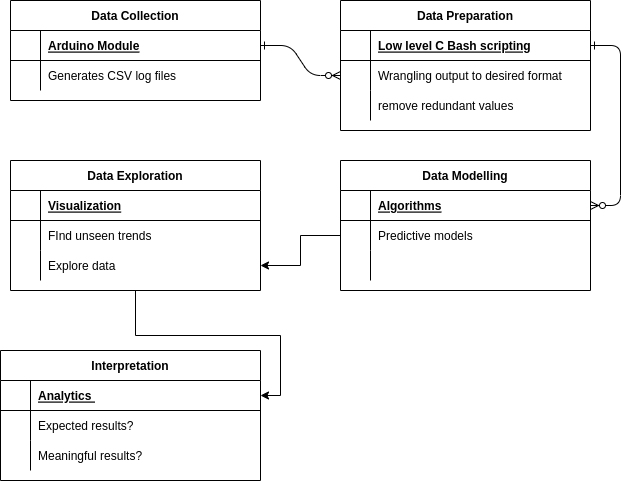
\includegraphics[width=0.7\linewidth]{Figures/data_analytics_process-steps}
	\caption{Data Analytics}
	\label{fig:dataanalyticsprocess-steps}
\end{figure}


\subsection{ Data Analysis}
The information gathered from the sensors will undergo scrutiny through tailored scripts. This analytical process will involve the generation of graphs aimed at evaluating and contrasting the performance of individual system components.

\subsubsection{Descriptive Analysis}
Before delving into the primary analysis, an exploratory data analysis will be conducted to ascertain the historical and current operational statuses of the components.

\subsubsection{Predictive Analysis}
Predictive analysis will be executed through the development of models, enabling the anticipation of potential issues. This includes the ability to forecast the need for replacement parts and estimate the time required for maintenance activities.

\subsubsection{Prescriptive Analysis}
The prescriptive analysis phase aims to provide strategic insights for achieving specific objectives. For instance, it may recommend measures to reduce the load by 5\% ultimately extending the service life of the components. This proactive approach is geared towards optimizing performance and ensuring the desired outcomes are achieved.
\newpage


\subsection{Sensor Placement}In the initial stages, We meticulously select suitable sensors and determine their optimal positions on the motor. The sensors are strategically placed to capture data from various motor components, including the stator, rotor, and bearings.
\subsection{Data Acquisition} We collect data from the motor during its operation, utilizing accelerometers or other specialized sensors. To ensure data accuracy, We sample at a sufficiently high frequency, allowing for the comprehensive capture of the desired frequency range.


\subsubsection{Preprocessing} After data collection, We apply various preprocessing techniques to the raw data to eliminate noise and artifacts. This involves filtering, normalization, and signal conditioning to enhance the overall quality and reliability of the data.
\subsubsection{Feature Extraction} Next, We extract relevant features from the preprocessed data. These features encompass a spectrum of characteristics, including time-domain features like RMS value and crest factor, as well as frequency-domain features such as spectral analysis and power spectral density. Advanced techniques like wavelet analysis and empirical mode decomposition may also be employed for extracting fault-related features.
\subsubsection{Fault Diagnosis}In the subsequent phase, We employ pattern recognition and machine learning algorithms to categorize the extracted features into different fault categories. To ensure the accuracy of the fault diagnosis models, the algorithms undergo training using labeled data derived from known fault conditions.


\subsubsection{Prognosis and Remaining Useful Life (RUL)} Utilizing regression analysis and prognostic algorithms, We estimate the remaining useful life of the motor. This involves tracking the degradation patterns of the motor over time and predicting potential failure points based on the extracted features and historical data.


\subsubsection{Prognostic Reporting} In the final steps, We generate comprehensive reports summarizing diagnosed faults, estimated remaining useful life, and recommended maintenance actions. These reports serve as valuable tools for maintenance personnel, aiding in the planning and execution of appropriate maintenance strategies, such as scheduling repairs or replacing the motor.